\section{Esercizio 20}
Polinomio di approssimazione ai minimi quadrati
\lstinputlisting[language=Matlab]{CodiceMatlab/Esercizio20/scriptEs20.m}
Eseguendo lo script si ottiene il seguente grafico:
\begin{figure}[h!]
    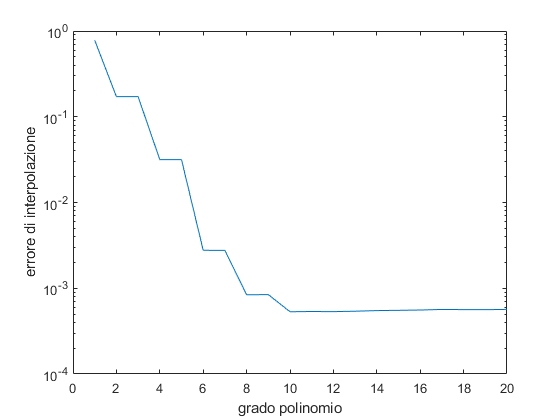
\includegraphics[scale=0.8]{CodiceMatlab/Esercizio20/graficoEs20.png}
    \caption{Grafico esercizio 20}
    \label{fig:es20}    
\end{figure}

Si può osservare  che l'errore decresce quasi esponenzialmente fino a circa $10^{-3}$, e quando il grado del polinomio m>=10, il grafico presenta un andamento costante.